
The Protégé plugin reuses much of the code written for the above-mentioned implementation. For the implementation, the information in the developer documentation \cite{protege5devdocs} has been consulted. Additionally, the implementation of other plugins \cite{ontodebug,protegepluginexamples} has been used as a basis for this plugin. It would have been desirable to share the same codebase between the two implementations, but some choices made for the prototype implementation were incompatible with its later use in the plugin. While Protégé is also using the OWL API, it is not using the latest version. Since for the implementation discussed in \cref{prototype} the latest OWL API version was used, and the two are not compatible, some changes had to be made. Further, the prototype has as dependencies the different OWL reasoners, this is a problem because those might not be included in Protégé, and bundling them with the plugin might cause conflicts if they are actually in Protégé already. For this reason, the implementation has been adapted to use the reasoner that is currently selected by the user in Protégé. Additionally, but less impactful, is also that Protégé uses an older version of Java than what has been used for the prototype implementation build for the evaluation. Three different ways to interact with the axiom weakening methods have been implemented in this plugin, we will show now each of them in turn.

\begin{figure}[ht]
  \centering
  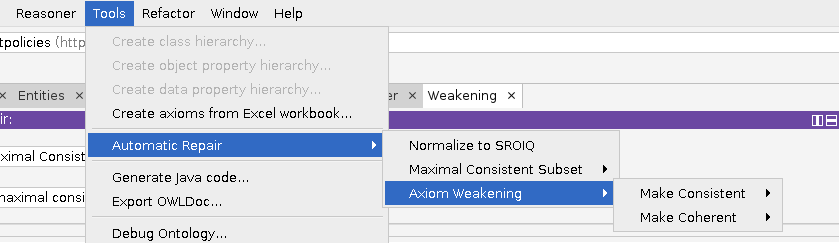
\includegraphics[width=\textwidth]{resources/protege-menu.png}
  \caption{Screenshot of the Protégé menu items added by the plugin.}
  \label{fig:protege-menu}
\end{figure}

To quickly apply the normalization or automatic repair algorithms, some menu items have been added by the plugin under ``Tools''. The first menu item, ``Normalize to SROIQ'', allows the quick application of the normalization, described in \cref{owl-to-sroiq}. Then there are two different repair algorithms for which menu entries have been added. The first, used by ``Maximal Consistent Subset'' selects as the repair a randomly selected maximal consistent subset. The second, used with ``Axiom Weakening'', is based on the algorithm listed in \cref{algo:repair-weaken}. For each of these two algorithms, the user may choose between making the ontology only consistent or making it also coherent. The repair for making the ontology coherent works analogously to the one for making the ontology consistent, except that the tests for consistency of the ontology are replaced with tests for coherence.

\begin{figure}[ht]
  \centering
  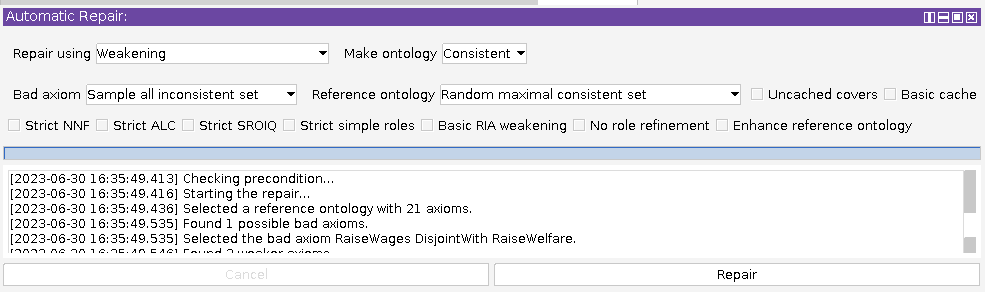
\includegraphics[width=\textwidth]{resources/protege-repair.png}
  \caption{Screenshot of the Protégé view added by the plugin, allowing for configuring and applying repairs algorithms.}
  \label{fig:protege-repair}
\end{figure}

The second method of interacting with the proposed axiom weakening repair algorithms is through a more detailed view added by the plugin. The user can select both the algorithm, e.g., by removal, using a maximal consistent set, using axiom weakening, etc., and the goal of the repair, i.e., consistency or coherence. Further, for some repair methods, options are made available. For the repair by weakening, all the flags and variations discussed in \cref{prototype} can be configured, as can be seen in \cref{fig:protege-repair}. Below the section for configuring the repair algorithm, a progress indicator and log have been placed. For long-running repairs, this is a valuable addition so that the user can see that the repair is still running. Another important feature that has been added specifically for the plugin is the ability to interrupt the repairs. To facilitate this functionality, the repair is started in a separate thread, and before every reasoner call, the implementation checks whether the thread has been interrupted, and if it has the repair is terminated by throwing an exception.

\begin{figure}[ht]
  \centering
  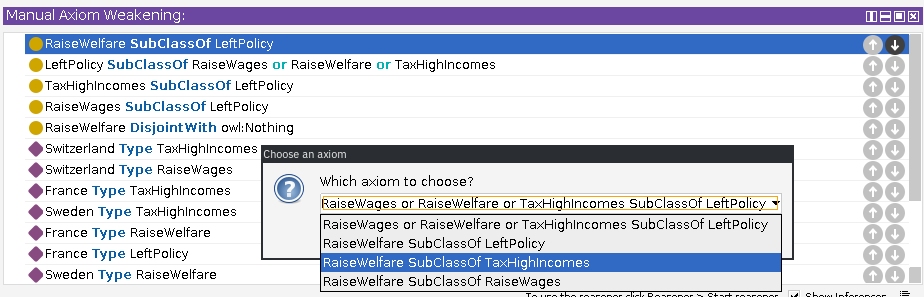
\includegraphics[width=\textwidth]{resources/protege-manual.png}
  \caption{Screenshot of the Protégé view added by the plugin, allowing for manually selecting axioms and weakening them.}
  \label{fig:protege-manual}
\end{figure}

Lastly, a view has been added that allows users to manually select how they want to weaken axioms. The view, depicted in \cref{fig:protege-manual}, shows a list of all axioms. The axioms are sorted by how frequently they appear in some minimal inconsistent subsets that are randomly sampled. The axioms that appear the most often are shown first, such that the axioms that are shown at the top of the list are the ones that would be selected by the automatic repair algorithm. The two buttons next to the axioms with the upward and downward arrows can then be used to, respectively, show weaker or stronger axioms. The user may choose one of these refined axioms to replace the original axiom.

